\newpage
\thispagestyle{endchapter}

\begin{tcolorbox}
\vspace{80pt}
	\lettrine{T}{here} were mixed feelings at the end of \emph{Povodni Mo\v{z}}: success in metres gained (2,267\,m in total) was acheived at a huge logistical and physical cost. The exciting exploration fronts still within reasonable distance from \passage{X-Ray} camp were now written off or pushed to their conclusion. The other leads lay further than ever before: either near the very deep end (\passage{Watership Down}) or a great caving distance to the south (\passage{Choke-a-Bloke}).

	Getting novices to navigate and successfully explore the cave is a particularly good metric to assess the outcome of an expedition. As new members have acquire a vast set of skills they can learn nowhere else (bolting, rigging, surveying), expeditions play a major role in the long term survival of the club: they refresh the pool of technical knowledge. We will not go far wrong by saying that the rich and unique baggage of experience and skills one brings back from deep alpine exploration is transferable to many other aspects of life.

	For that reason, the format of the 2016 expedition was heatedly discussed soon after we came back to the UK. Wondering how best to readjust our aims and targets without losing the opportunity to find new passage, we started looking beyond \passage[cave]{Vrtnarija}, to potential new areas of the mountain, and toyed with the idea of abandoning the underground camp. Luckily, a solution presented itself, coming in the form of a celebratory message from a well known corner of the Alps...

	The long awaited connection between \passage[cave]{Monatip} - \passage[cave]{Primadona} system and \passage{System} \passage{Migovec} was forged during the usual October Super Action run by the JSPDT. Navigating through a system of shallow, horizontal galleries filling an area of mountain hitherto unexplored, the lucky explorers unexpectedly connected with the SE end of \passage{NCB} passage, thus confirming \passage[cave]{Sistem Migovec}'s status as longest cave in ex-Yugoslavia.

	
\end{tcolorbox}
	\backgroundsetup{	scale=1,
					color=black,
					opacity=1,
					angle=0,
					contents={%
  						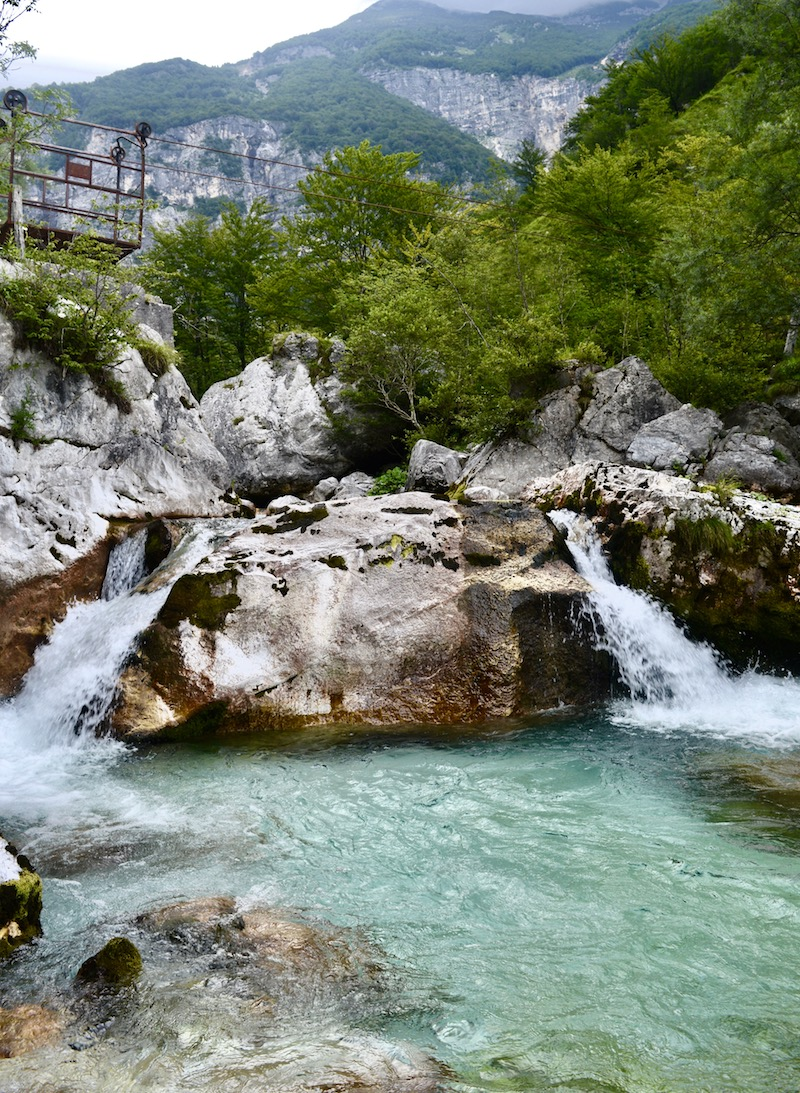
\includegraphics[height=\paperheight]{images/backgrounds/tolminka_at_crossing__2_.jpg}
  					}
	}
\BgThispage